\section{Evaluation}
\label{sec:eval}

We've evaluated Tutamen in a variety of scenarios using the
applications described in \S~\ref{sec:apps}. In this section, we
discuss both our existing Tutamen deployment as well as the
performance characteristics of our Tutamen prototype.

\subsection{Deployment}
\label{sec:eval:deployment}

We've deployed a group of Tutamen servers, each either hosted locally
or by an independent third party in order to gain geospatial,
geopolitical, and administrative diversity. Our current Tutamen
deployment includes three access control and storage server pairs,
across wish we can shard both secrets and access control duties:

\begin{packed_desc}
\item[Paris, France:] Scaleway~\cite{scaleway} C2S instance\footnote{Bare
  metal, 4-core, 8GB, Intel Atom C2550}
\item[North Virginia:] AWS EC2~\cite{amazon-ec2} c4.large
  instance\footnote{VM, 2-core, 3.75GB, Intel Xeon E5-2666}
\item[Boulder, CO:] Self-hosted instance\footnote{VM, 4-core, 4GB
  virtual, Intel Xeon E3-1245}
\end{packed_desc}

We've utilized our experimental Tutamen deployment to manually store
secrets via the Tutamen CLI, to store encryption keys for our FuseBox
app, and to store encryption keys for our LUKS and our QCOW2 full-disk
encryption systems. In each case, Tutamen has allowed us to realize
use cases not easily attainable before such as the use of full disk
encryption on headless servers and the sharding of sensitive files via
Dropbox. This deployment demonstrates Tutamen's usefulness as an
enabler of previously unattainable functionally in a manner that also
minimizes the need for third party trust. While Tutamen is still a
prototype, our experience utilizing it thus far leads us to believe it
provides a well-designed architecture capable of supporting a wide
range of practical secret-storage applications.

\subsection{Performance}
\label{sec:eval:perf}

\begin{figure*}[thb]
  \centering
  \begin{subfigure}[t]{0.48\textwidth}
    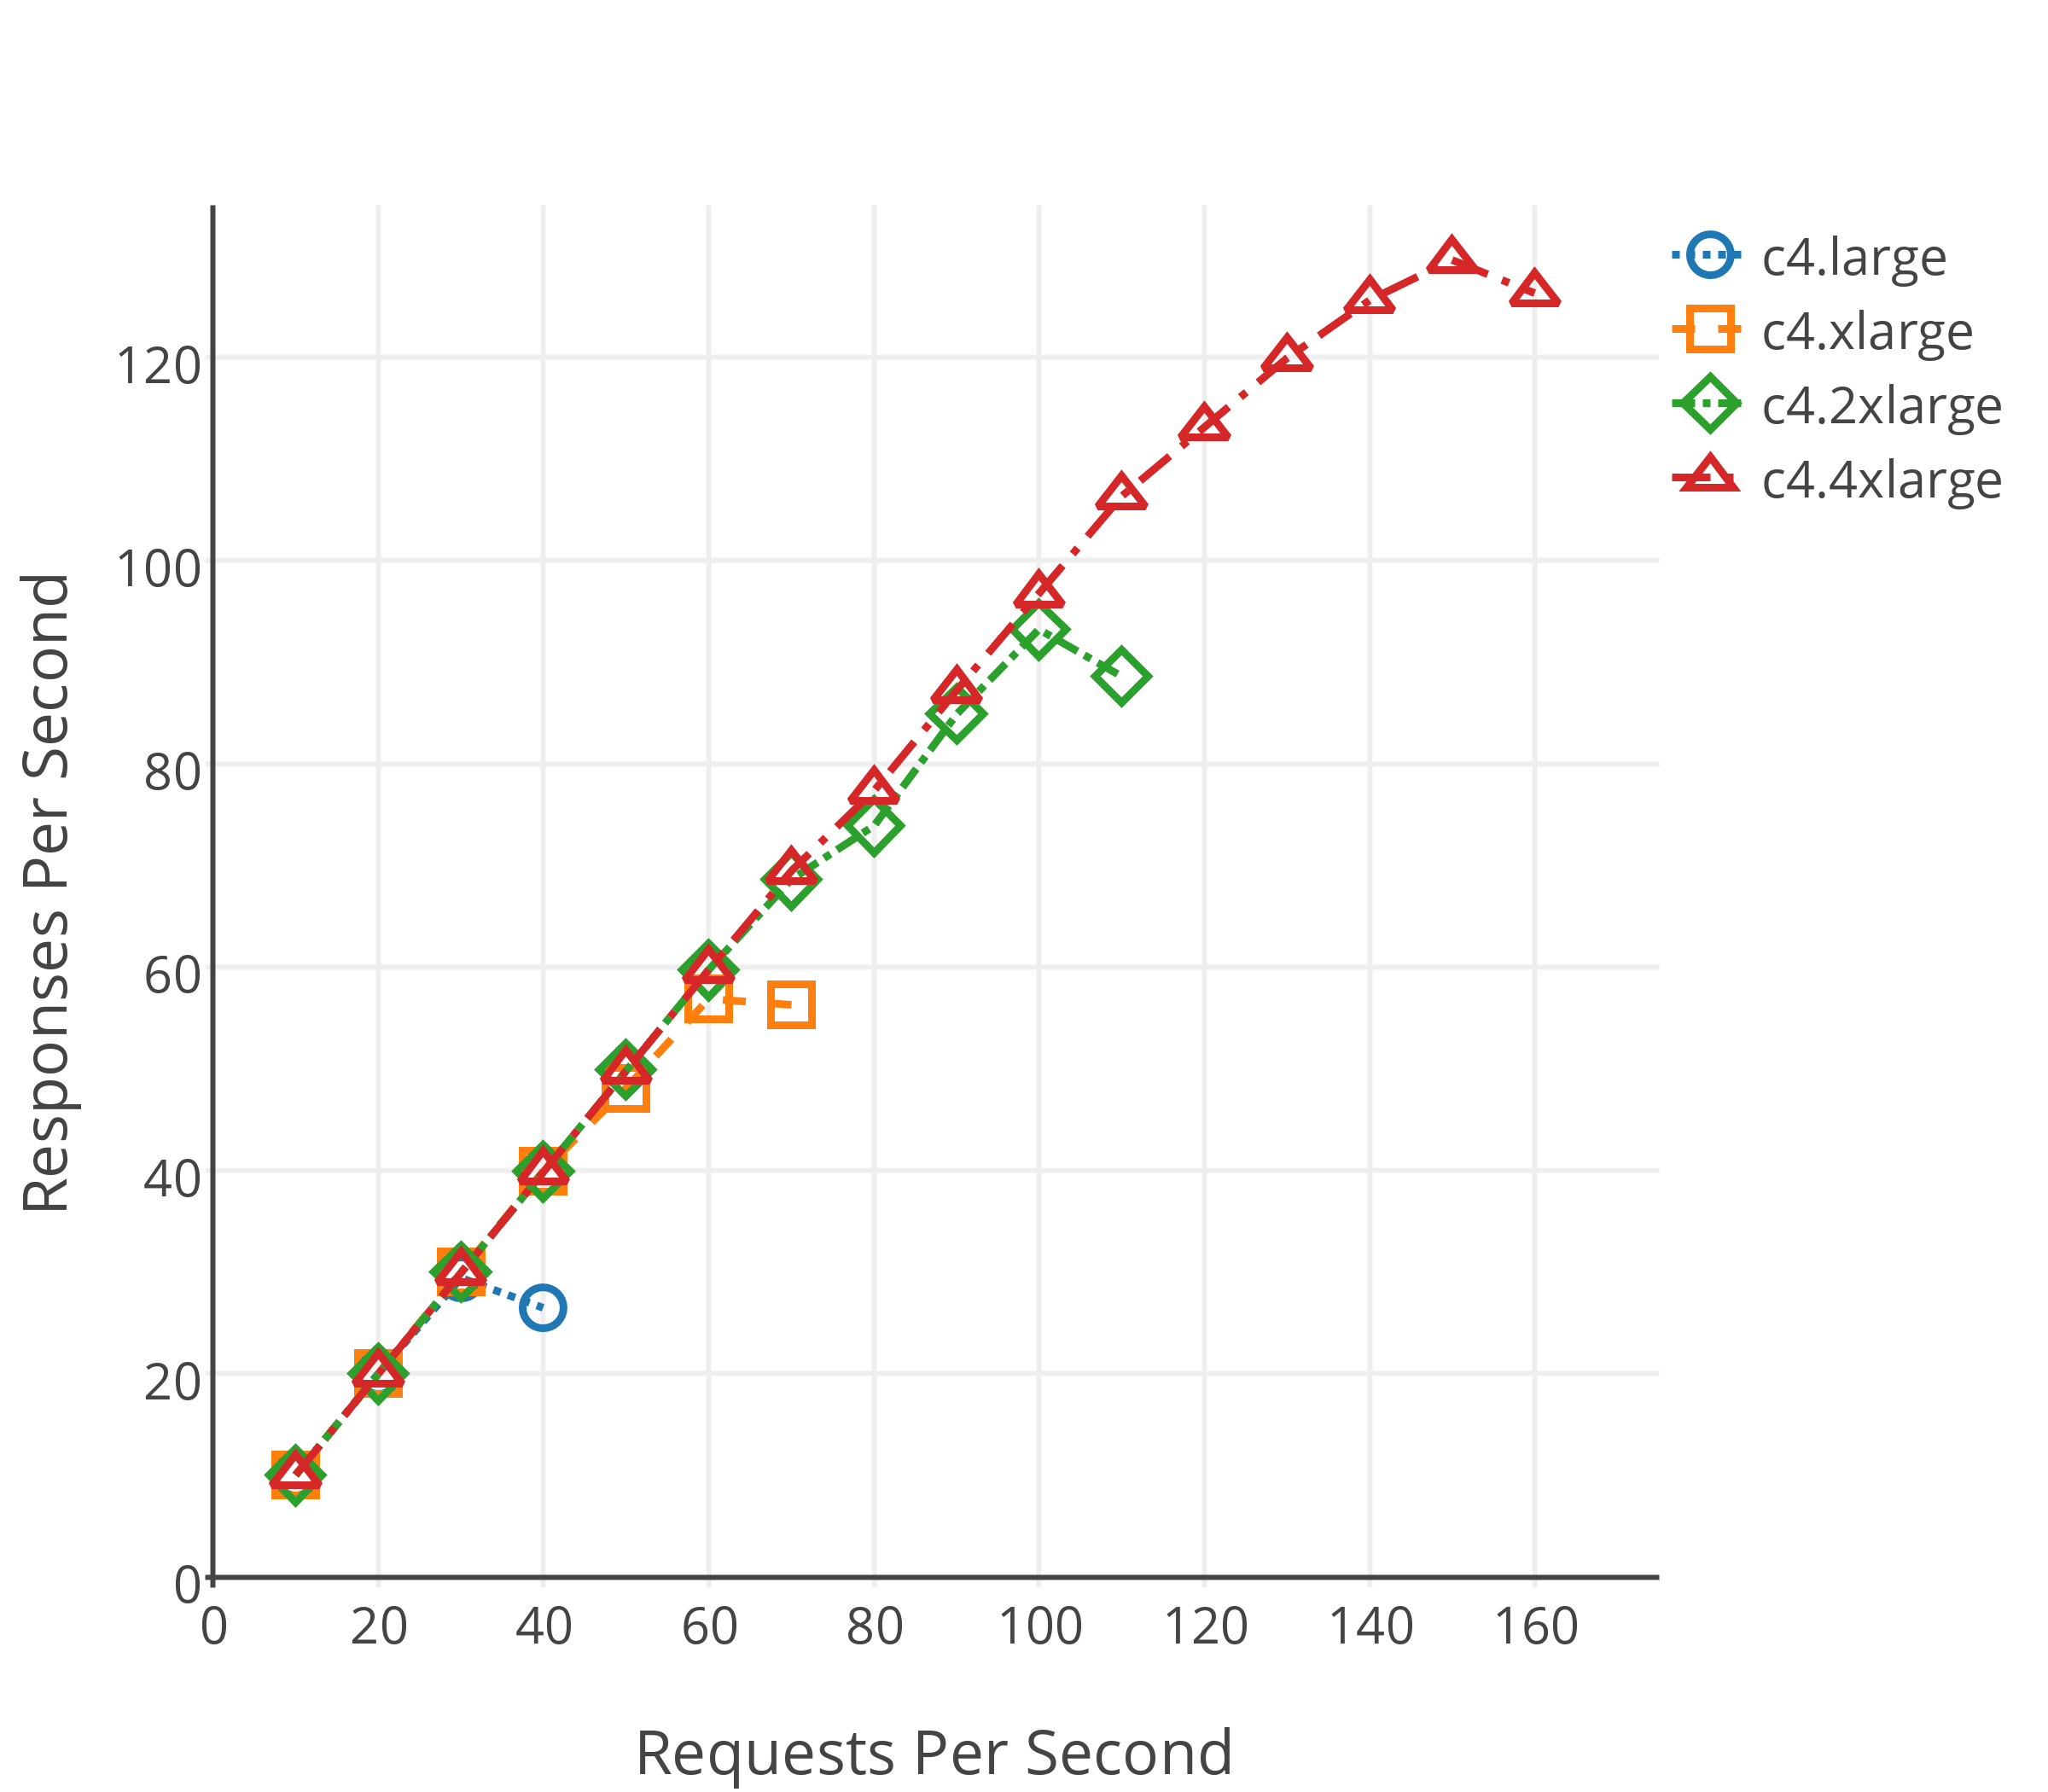
\includegraphics[width=\textwidth]{./figs/png/get_ac_auth_comp_chart.png}
    \caption{AC Server -- Get Authorization Token}
    \label{fig:eval:scaleup:gettoken}
  \end{subfigure}
  ~
  \begin{subfigure}[t]{0.48\textwidth}
    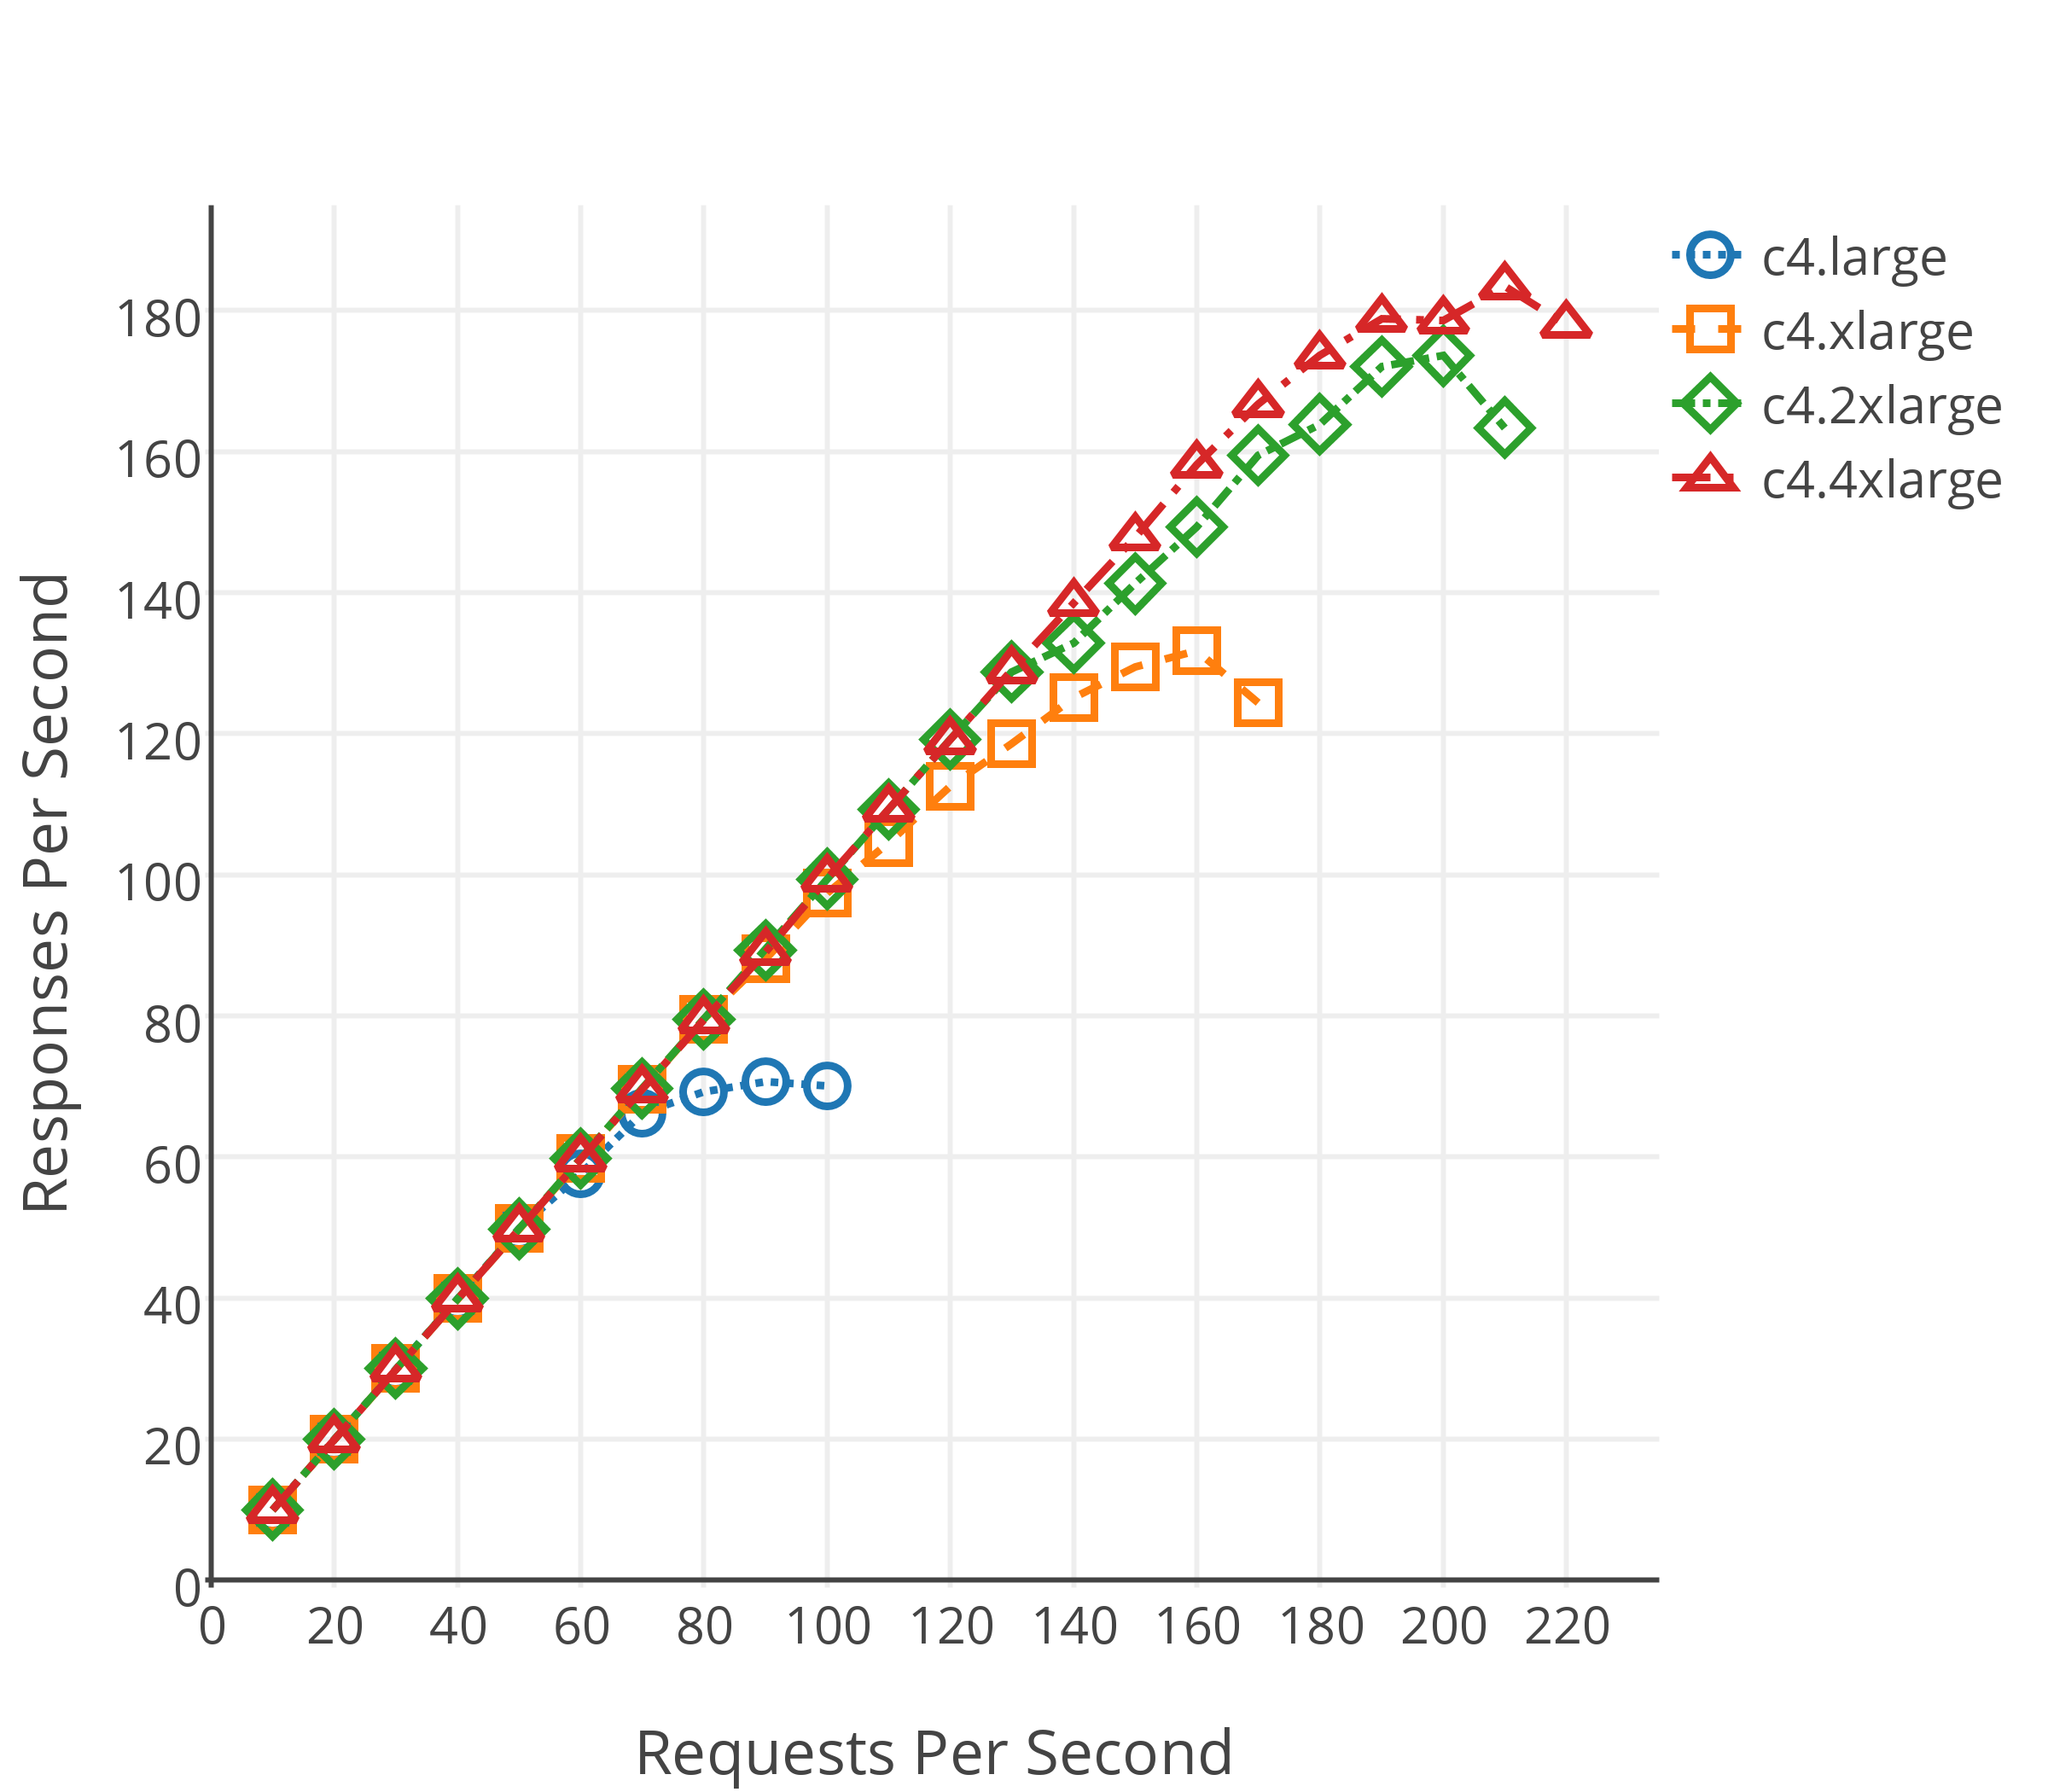
\includegraphics[width=\textwidth]{./figs/png/get_ss_secret_comp_chart.png}
    \caption{Storage Server -- Fetch Secret}
    \label{fig:eval:scaleup:getsecret}
  \end{subfigure}
  \caption{Scale Up Performance of Tutamen Servers on Amazon EC2 Gen4
    Compute-Optimized Instances}
  \label{fig:eval:scaleup}
\end{figure*}

All of the scenarios in which we've used Tutamen thus far share the
quality that they require a low rate of secret storage/retrieval
requests. E.g. FuseBox requires only a single secret store per file
create operation and a single secret lookup per file open
operation. The full disk encryption schemes are even less demanding,
requiring only a single lookup per system boot. Since our current
deployment has easily supported the needs of our existing Tutamen
users and applications, we have not yet had a need to optimize our
Tutamen deployment for performance. Nonetheless, we have performed a
number of performance measurements in order to better understand the
scaling and bottlenecks of the Tutamen system and to target future
performance enhancements.

Figure~\ref{fig:eval:scaleup} shows the response vs request rates of
single access control and storage server deployment across a range of
increasingly powerful Amazon EC2 compute-optimized instances. The
curve for each instance tops out once the server reaches its maximum
processing capability. Increasing the request rate beyond that point
only serves to increase the response latency, and eventually leads to
diminished performance due to server thrashing. Thus, we only graph
through the first data point that shows a decrease in response rate
relative to previous data point, and this that represents the
asymptotic performance limit of each flavor.

Figure~\ref{fig:eval:scaleup:gettoken} shows performance of a stream
of ``Get Authorization Token'' requests to a single Tutamen Access
Control server for a verifier that requires only account membership
(e.g. no authenticator modules). The max request rate scales fairly
linearly with the number of CPU cores, ranging from around 30 RPS on a
c4.large to around 130 RPS on a c4.4xlarge. Processing authorization
token requests tends to be the most computationally difficult Tutamen
operation: the process requires verifying both cryptographic
assertions (e.g. a client certificate via the account ID) as well as
loading and verifying each authenticator module (where
required).\footnote{Processing authorizations can also incur
  human-scale delays far in excess of the computational limits, as in
  cases where an SMS authenticator requires a human to receive and
  then respond to a text message. Tutamen clients must thus account
  for the possibility of significant delays when requesting tokens,
  generally via timeouts or asynchronous callbacks.}
Figure~\ref{fig:eval:scaleup:getsecret} shows a similar set of curves
for a stream of request to fetch a secret from a Tutamen storage
server. As in the access control case, these operations scale linearly
with the number of CPU cores, up until the point where they top out
via the diminishing return of a c4.4xlarge instance relative to a
c2.2xlarge instance. While we have not fully determined the exact
cause of this limit, we believe it is a combination of our Python test
client itself being only capable of generating ~180 TLS requests per
second and the fact that the Redis database starts to reach the limit
of the instances I/O performance around this point, leading us to
become I/O instead of CPU bound. It should be noted that the request
secret operation requires significantly fewer computational resources
than the ``get token'' operation, leading to a performance range of
~70 RPS to ~180 RPS.

\begin{figure*}[thb]
  \centering
  \begin{subfigure}[t]{0.48\textwidth}
    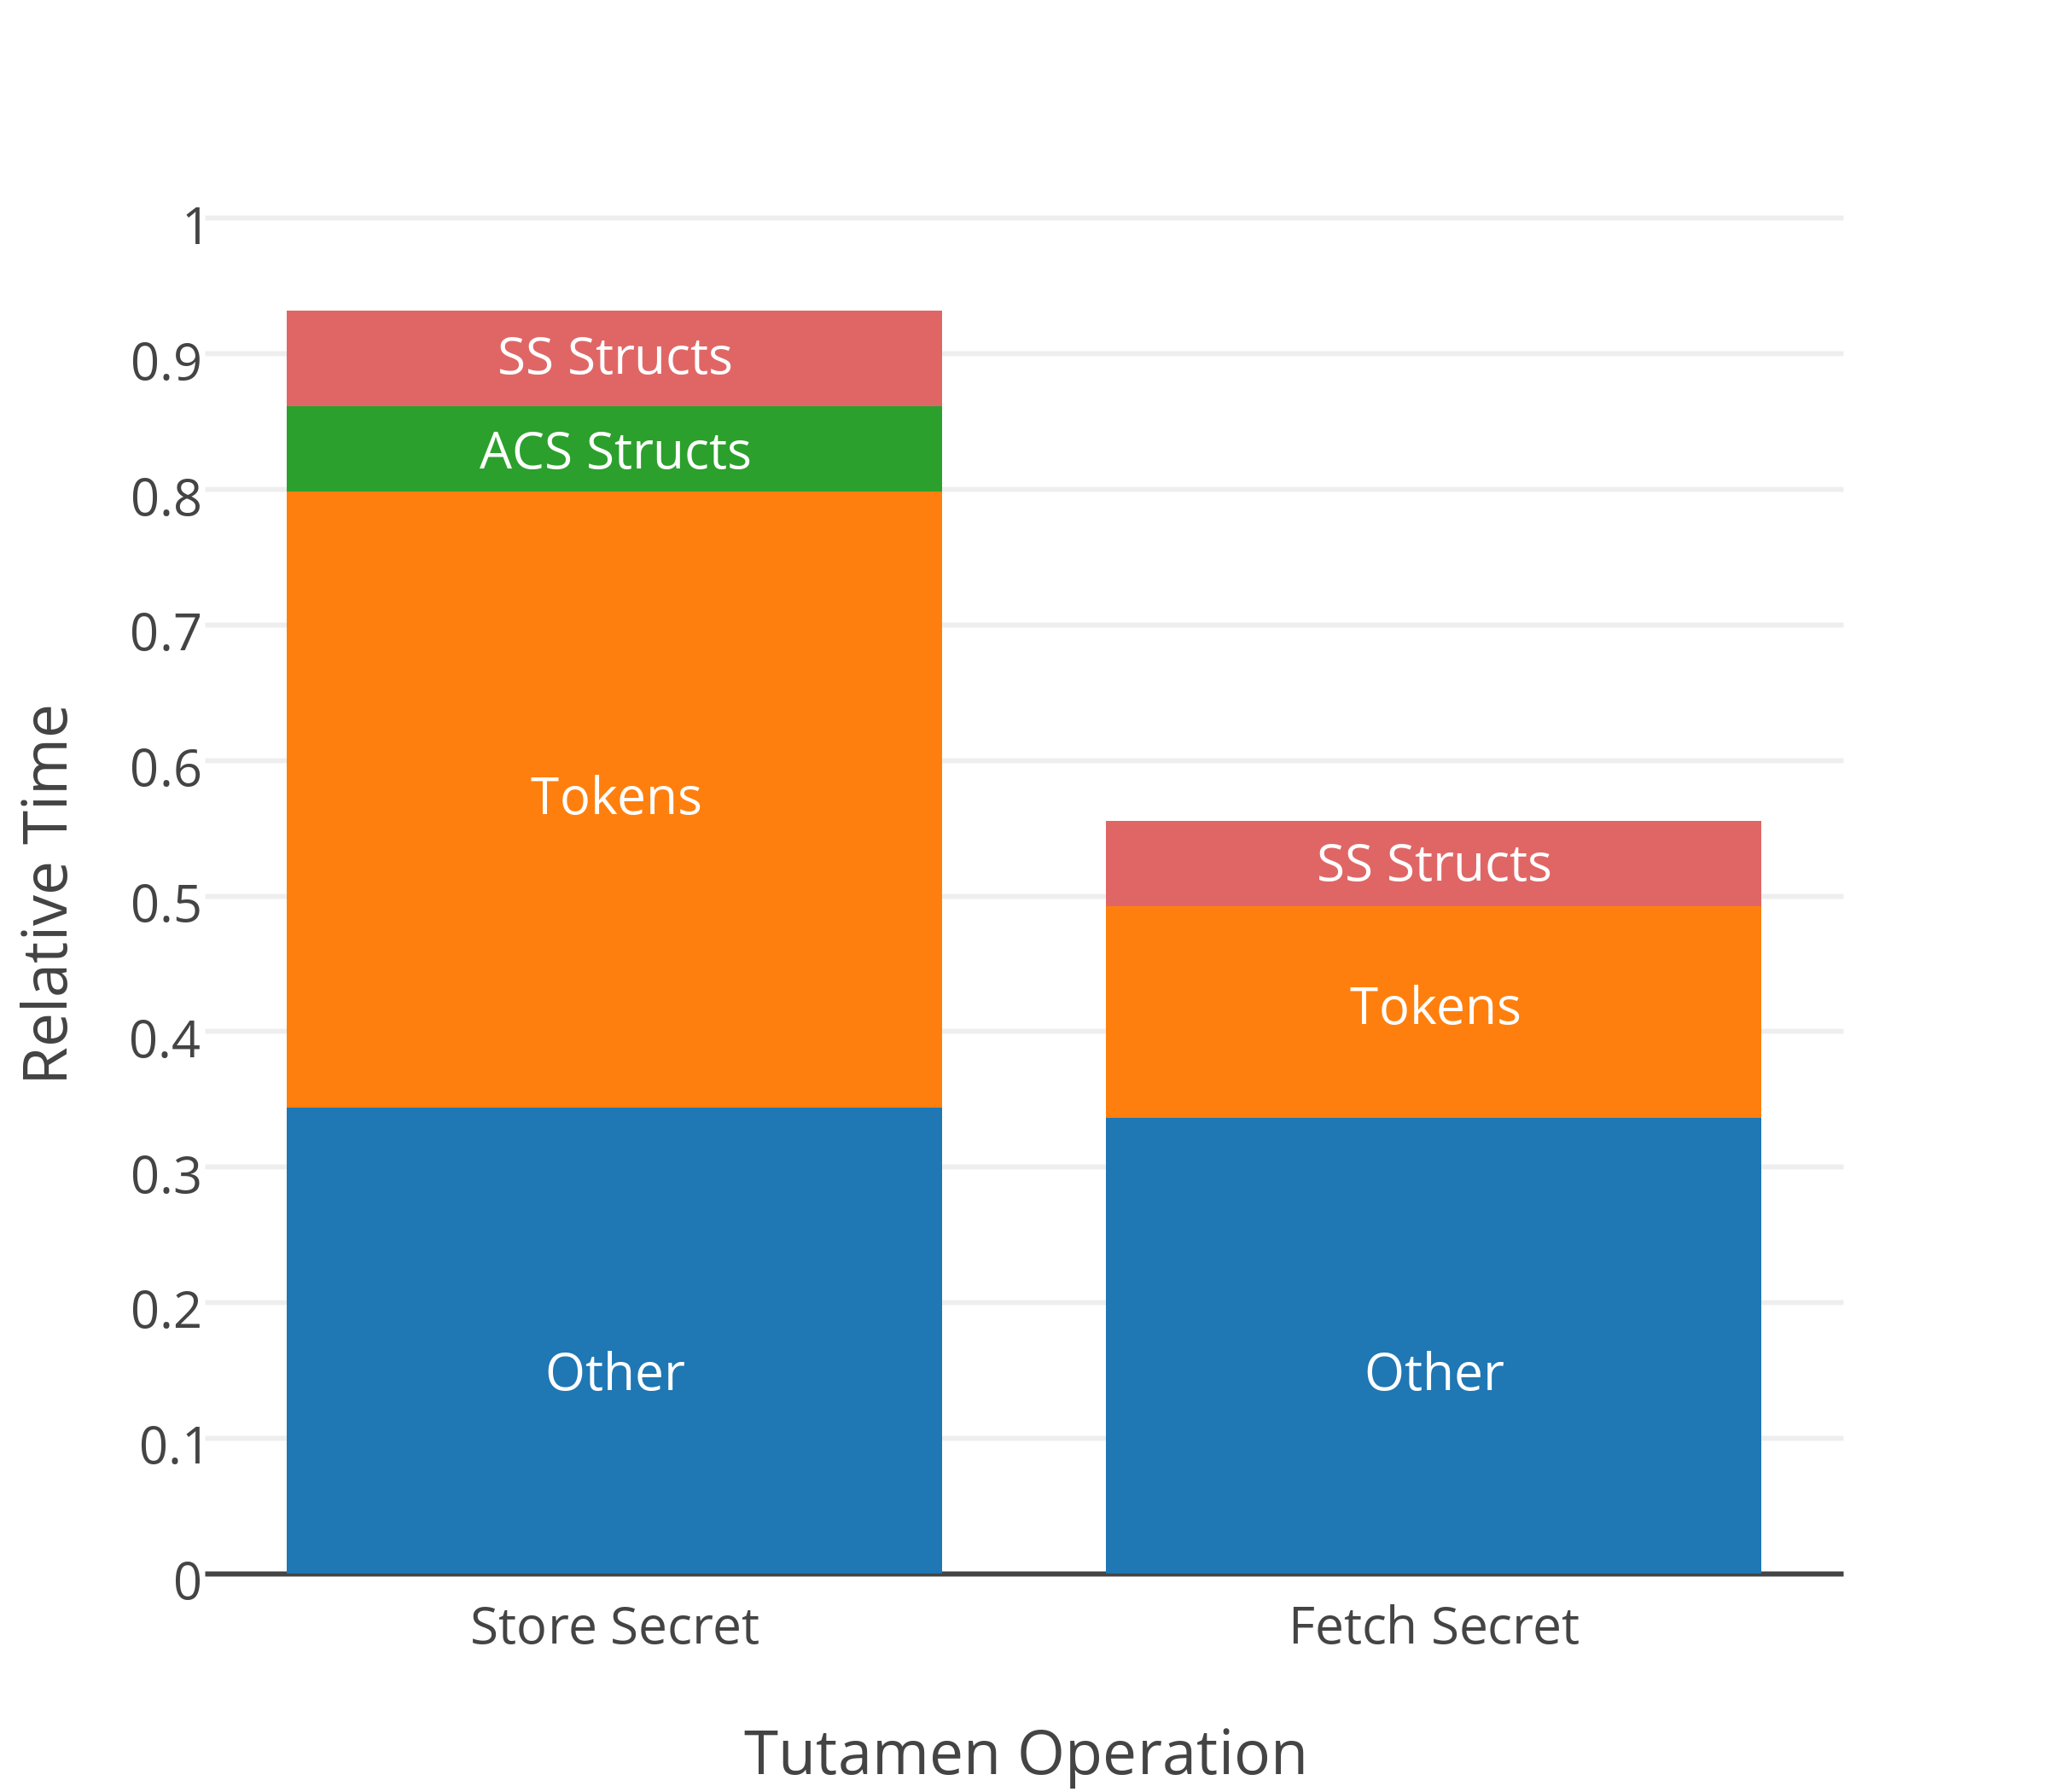
\includegraphics[width=\textwidth]{./figs/png/timing_bars_chart.png}
    \caption{Relative Time Spent Processing Store and Fetch
      Operations}
    \label{fig:eval:rel:secret}
  \end{subfigure}
  ~
  \begin{subfigure}[t]{0.48\textwidth}
    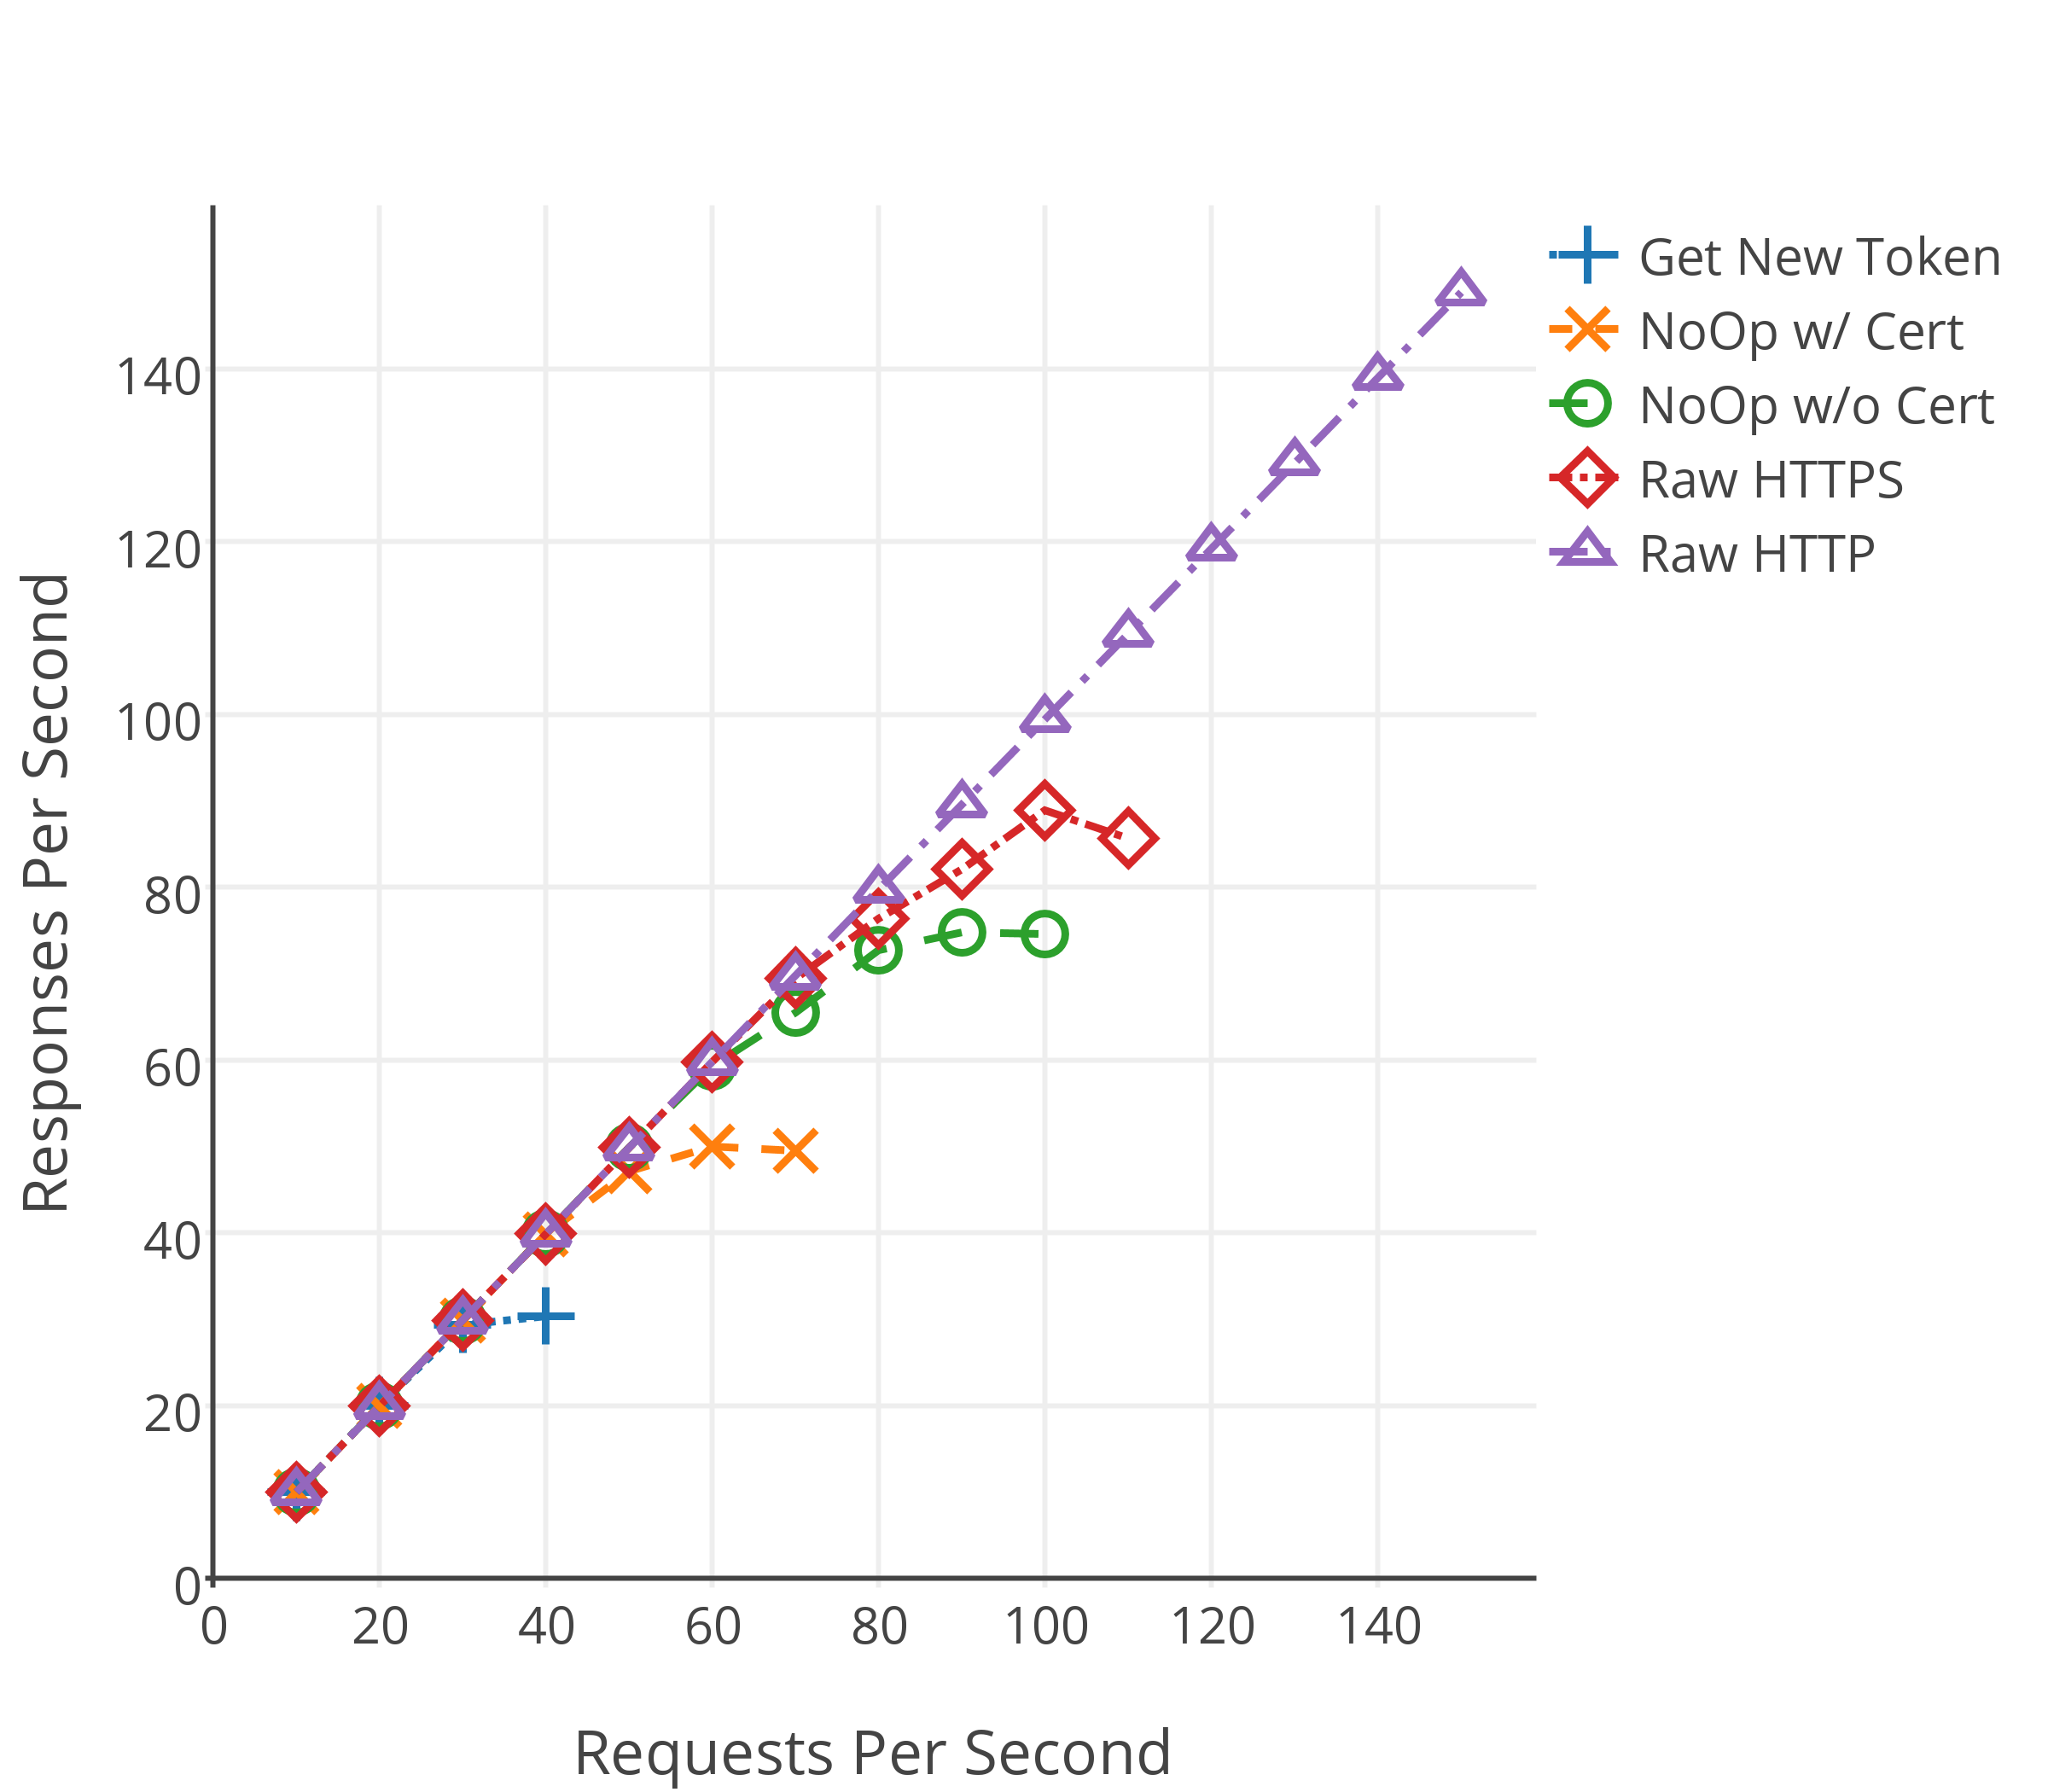
\includegraphics[width=\textwidth]{./figs/png/get_ac_auth_breakdown_chart.png}
    \caption{Relative Performance of Tutamen AC Server Operations}
    \label{fig:eval:rel:acops}
  \end{subfigure}
  \caption{Timing and Performance Comparison of Tutamen Server
    Operation Sub-components}
  \label{fig:eval:rel}
\end{figure*}

Figure~\ref{fig:eval:rel:secret} shows the breakdown of the relative
time required to complete two of the most common Tutamen operations:
storing a new secret and retrieving a previously stored secret. We
profiled the amount of time the Tutamen CLI application spent
performing various parts of each of these two Tutamen operations. In
both operations, the bulk of the server-related runtime is spent
requesting and retrieving the authorization tokens required to
complete the associated operations. In the secret creation case, five
tokens are required.\footnote{I.e. one token to create the permissions
  for a new verifier, one token to create a new verifier itself, one
  token to create permissions for a new collection, one token to
  create the collection itself, and one token to store a new secret
  within the collection.} In the secret read case, only a single token
is required.\footnote{I.e. to read a secret within the collection.}
The remainder of the server-related time is spent either creating AC
and storage data structures (e.g. verifiers, collections, etc), or
reading existing data structures. The ``other'' time is spent reading
the Tutamen config files, loading the necessary client certificates,
and dealing with the overhead required to setup the TLS connections
and interpret the Python-based CLI.
 
Figure~\ref{fig:eval:rel:secret} shows the response vs request rate
for a standard token request operation, two ``No-Op'' AC API
operations (one that sends and verifies the client TLS certificate and
one that does not), and raw Apache HTTPS and HTTP page loads as
preformed on an Amazon EC2 c4.large instance. As these curves show,
token verification on such an instance tops out around 30 RPS. The
null AC API operation with client certificates tops out around 50 RPS,
and the null operation without client certificates tops out at about
75 RPS. Raw HTTPS tops out around 90 RPS. HTTP topped out around 550
rps (curve truncated for viewability). Our Tutamen prototype is thus
primarily limited by the TLS overhead required to serve the
application and verify client certificates. Token verification itself
also incurs additional computational requirements, including
cryptographic signing operations. Finally, the data retrieval itself
incurs some overhead.

While the current Tutamen performance has been sufficient for our
in-house needs, we have planes to optimize and increase the
performance of our Tutamen deployment. On the server-side, Tutamen is
designed to allow both horizontal and vertical scaling, and we foresee
large deployments overcoming both the computational and I/O barriers
of our current deployment through a mix of balancing requests across
multiple backend instances (i.e. to overcome database and I/O limits
of single instance) and the use of more powerful processing
capabilities (e.g. cryptographic accelerators). We also have plans to
streamline the cryptographic code as well as the database abstraction
layer to decrease Tutamen's computational and I/O requirements. On the
client, we also have plans to take advantage of Tutamen's support for
long-lived (e.g. minutes to hours vs seconds) tokens to decrease the
frequency with which clients must make requests to the Tutamen AC
server. Finally, we also have plans to amend the Tutamen protocol to
allow for batching multiple token and storage sever requests together
to decrease the ratio of authentication overhead to useful work
possible in a single round trip request. We're believe a combination
of these techniques would allow us to significantly increase the
performance of our Tutamen deployment with only moderate additional
effort.

%%  LocalWords:  Tutamen Tutamen's verifiers authenticators SMS Xeon
%%  LocalWords:  authenticator HTTPS Redis viewability Scaleway QCOW
%%  LocalWords:  FuseBox xlarge CPUs golang AWS
